\chapter{Projeto Conceitual do Produto}

\section{Características gerais}

 O projeto do foguete tem como objetivo alcançar distâncias predefinidas de dez, vinte e trinta metros, que podem ser selecionadas eletronicamente a distância. Diante disso, o foguete deve ser reutilizado durante os três lançamentos, necessitando, assim, de uma estrutura consolidada e resistente, que assegure a firmeza da estrutura e proteja os componentes eletrônicos. O foguete será lançado a partir de uma base com ângulo fixo durante os três lançamentos. A partir disso, para a variação da distância, será necessário ajustar a pressão de lançamento. Sob esse viés, para o gerenciamento de todas essas necessidades, a equipe de eletrônica desenvolveu sistemas de armazenamento de dados e telemetria, capazes de registrar as informações necessárias para lançamentos precisos, além de permitir o acionamento remoto do lançamento.

Ademais, a equipe de software desenvolveu algoritmos cruciais para o processamento dos dados coletados pelos sistemas eletrônicos, que permitem o ajuste da distância de lançamento. Também foi criada uma interface que possibilita a visualização dos dados do lançamento e dos sensores de forma simples e rápida.

Portanto, com todos esses sistemas desenvolvidos, o foguete é capaz de suportar os lançamentos, além de fornecer visualizações digitais dos dados de maneira clara e acessível.

%\textcolor{red}{Descrever produto de forma geral. Apresentar itens teóricos sobre o projeto a serem aprofundados ou detalhados oportunamente.}

%\textcolor{red}{Apresentar e explicar a Estrutura Analítica do Projeto (EAP), tomando cuidado com a legibilidade da imagem. Se necessário, coloque a EAP dentro do comando ``\textsf{\textbackslash begin\{landscape\} \textbackslash end\{landscape\}}'' para que ela seja apresentada em uma página deitada.}

\begin{landscape}

\begin{figure}
    \centering
    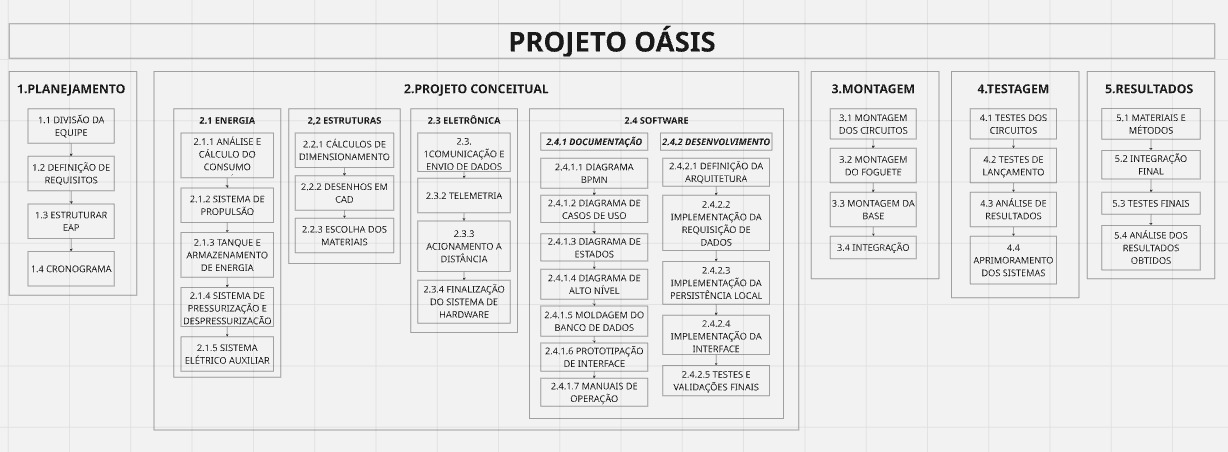
\includegraphics[width=1\linewidth]{editaveis/figuras/EAP_ProjetoOasis.jpeg}
    \caption{Estrutura analítica de projeto}
    \label{fig:enter-label}
\end{figure}

\end{landscape}


\begin{landscape}
\section{Descrição de \textit{software}}
\subsection{Diagrama BPMN}

O BPMN é uma notação que oferece modelos e representações gráficas para visualizar de forma clara os fluxos de atividades e as etapas dos processos dentro de ambientes empresariais e projetos. Seu principal foco é fornecer diagramas de fácil compreensão para todas as pessoas envolvidas, garantindo que todos os membros do grupo estejam alinhados aos objetivos do projeto.

\begin{figure}[H]
    \centering
    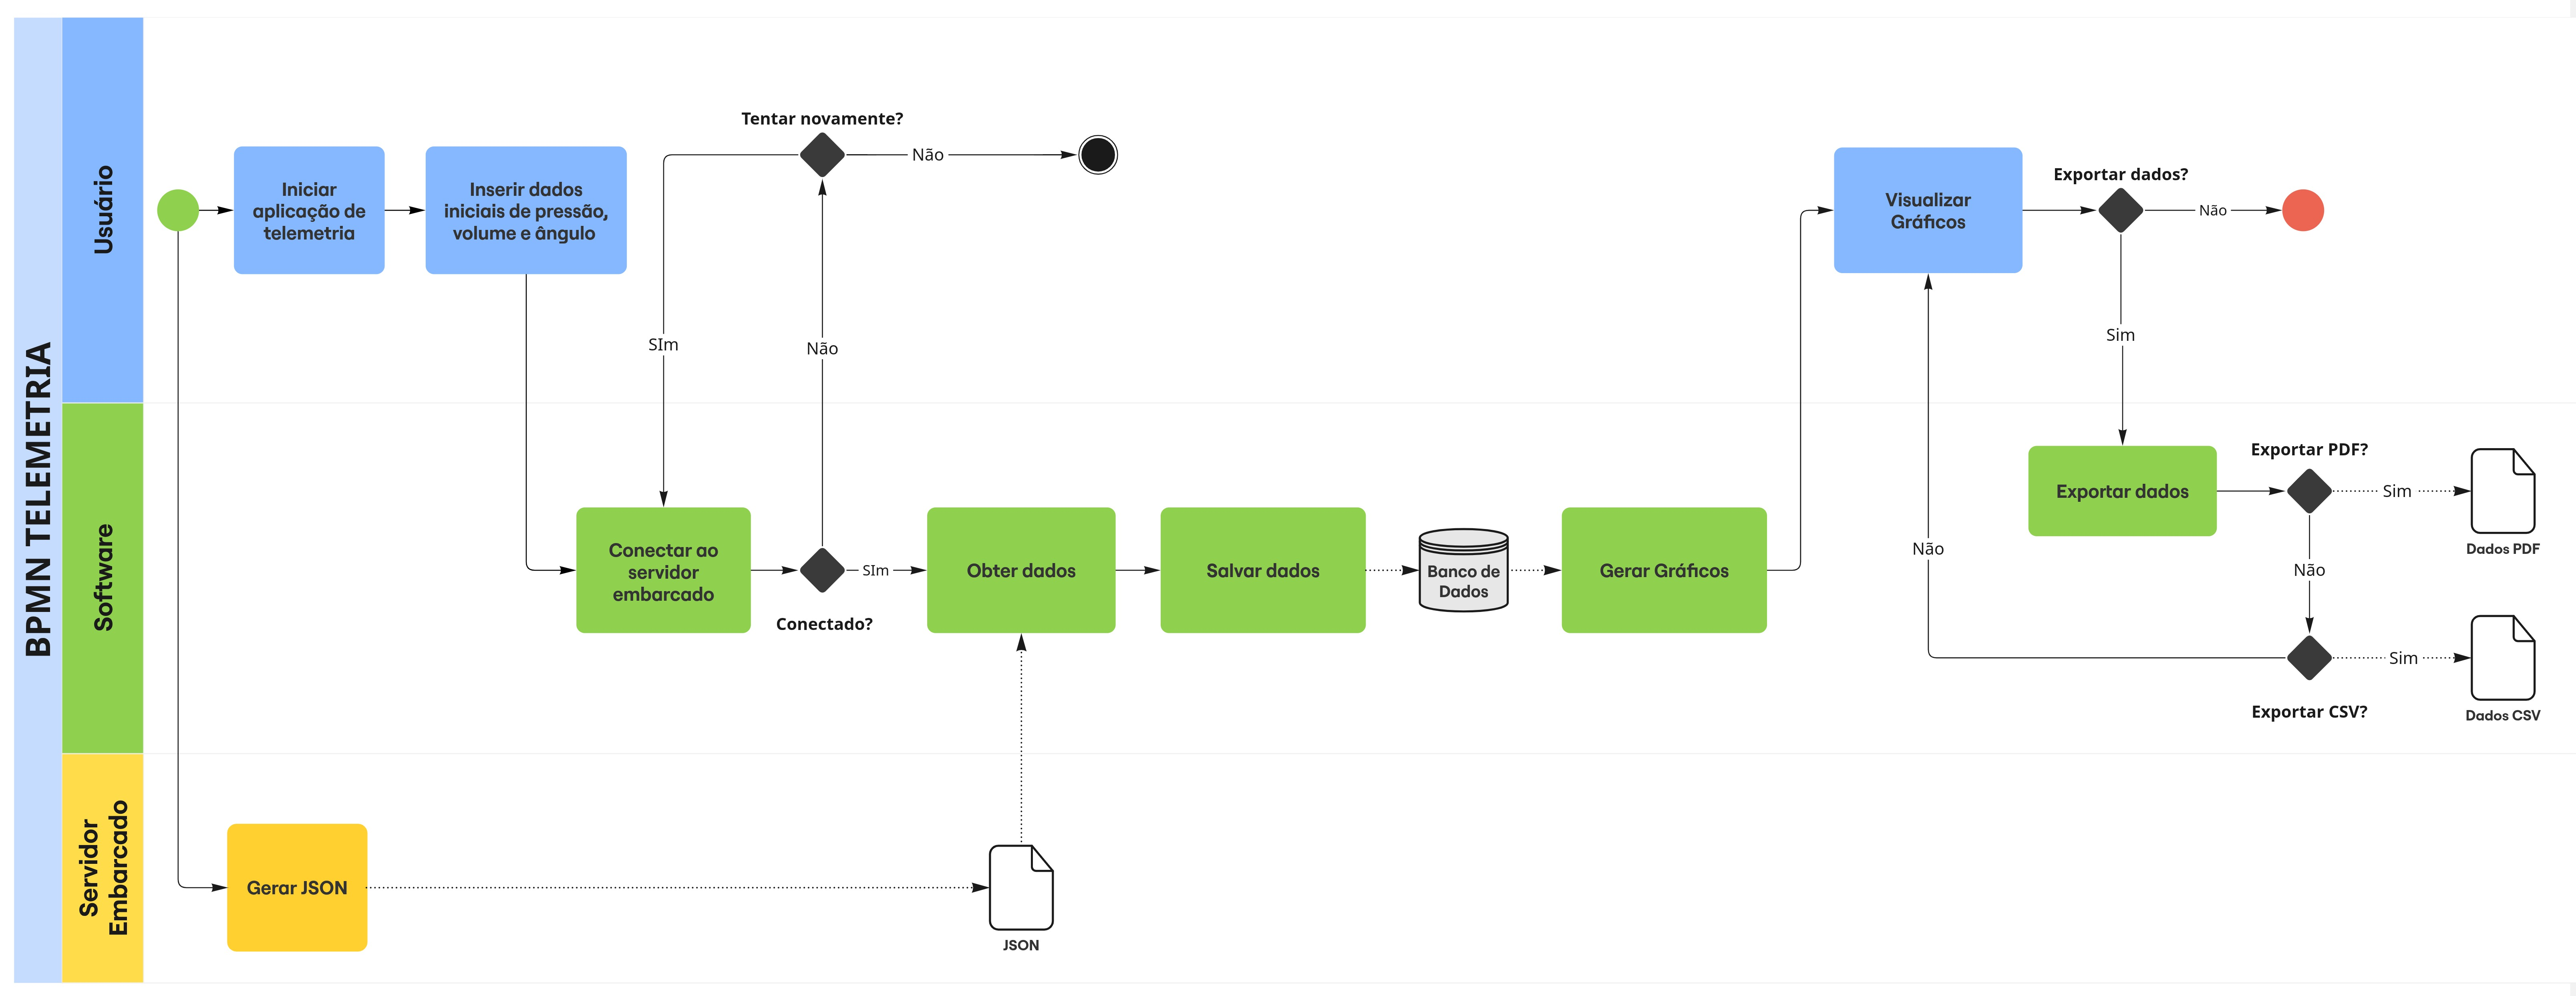
\includegraphics[width=1\linewidth]{editaveis/figuras/bpmn.jpg}
    \caption{Diagrama BPMN}
    \label{fig:enter-label}
\end{figure}
\end{landscape}

\subsection{Backlog Funcional}
O backlog funcional é uma lista organizada de funcionalidades que um sistema deve implementar para atender às necessidades dos usuários. Ele serve como um guia para o desenvolvimento do software, definindo o que precisa ser feito, por que e para quem.

O backlog funcional do projeto Oásis segue o formato de histórias de usuário, representando os requisitos funcionais sob a perspectiva do usuário final. Elas seguem um formato padrão:

\textit{“Eu, como [tipo de usuário], quero [ação] para [benefício].”}

Esse formato ajudará a equipe de software a entender quem vai usar a funcionalidade, o que a pessoa deseja fazer e por que tal funcionalidade é importante.

Os requisitos funcionas foram classificados utilizando o MoSCoW, técnica utilizada para definir a prioridade de cada funcionalidade no backlog.

O operador representa a pessoa que utilizará diretamente o sistema.

\setlength{\extrarowheight}{2pt}

\begin{longtable}{|>{\centering\arraybackslash}m{2cm}|
                    >{\centering\arraybackslash}m{2.7cm}|
                    >{\centering\arraybackslash}m{1cm}|
                    >{\centering\arraybackslash}m{6cm}|
                    >{\centering\arraybackslash}m{2cm}|}
  \hline
  \textbf{Épico} & \textbf{Feature} & \textbf{ID} & \textbf{História de Usuário} & \textbf{MoSCoW} \\
  \hline
  \endfirsthead
  
  \hline
  \textbf{Épico} & \textbf{Feature} & \textbf{ID} & \textbf{História de Usuário} & \textbf{MoSCoW} \\
  \hline
  \endhead

E01 Coleta de Telemetria
    & F01: Conexão ao servidor embarcado & US01 & Eu, como operador, quero conectar o software ao servidor embarcado no foguete para iniciar a leitura dos dados de voo. & Must \\
  \cline{2-5}
    & F02: Requisição de dados JSON & US02 & Eu, como operador, quero requisitar os dados do voo em formato JSON para processá-los no sistema. & Must \\
  \cline{2-5}
    & F03: Persistência dos dados & US03 & Eu, como operador, quero salvar os dados coletados em um banco de dados para uso posterior e comparação entre lançamentos. & Must \\
  \hline

E02 Análise de Voo
    & F04: Visualização gráfica & US04 & Eu, como operador, quero visualizar gráficos de aceleração e velocidade para analisar a trajetória do foguete. & Must \\
  \cline{2-5}
    & F05: Indicadores de desempenho & US05 & Eu, como operador, quero ver o tempo de voo e distância final para verificar se os requisitos de alcance foram atendidos. & Should \\
  \cline{2-5}
    & F06: Análise comparativa & US06 & Eu, como operador, quero comparar os dados entre os três lançamentos para calibrar o foguete com base nos resultados. & Could \\
  \hline

E03 Interface com o Usuário
    & F07: Dashboard interativo & US07 & Eu, como operador, quero navegar entre as telas de conexão, gráficos e análise para usar o sistema com facilidade. & Should \\
  \cline{2-5}
    & F08: Exportação dos dados & US08 & Eu, como operador, quero exportar os dados dos lançamentos em CSV para realizar análises externas. & Could \\
  \cline{2-5}
    & F09: Exportar relatório em PDF & US09 & Eu, como operador, quero exportar os gráficos e dados em formato .PDF para documentar o desempenho do foguete. & Could \\
  \hline

E04 Calibração de Trajetória
    & F10: Ajuste por parâmetros & US10 & Eu, como operador, quero visualizar os dados de entrada como pressão, volume e ângulo para entender seu impacto no desempenho. & Should \\
  \hline

\end{longtable}



\renewcommand{\arraystretch}{1.2} % Espaçamento entre linhas

\subsection{Backlog Não-Funcional}

O \textbf{Backlog Não-Funcional} reúne os requisitos que não dizem respeito diretamente às funcionalidades do sistema, mas que garantem sua qualidade, desempenho, segurança, usabilidade e outros atributos essenciais. Esses requisitos asseguram que o sistema funcione de maneira eficaz, seja confiável, seguro, escalável e mantenha a integridade dos dados e da experiência dos usuários.

\subsubsection*{Requisitos}

\begin{longtable}{|p{5cm}|p{3cm}|p{7cm}|}


\hline
\textbf{Requisito} & \textbf{Tipo} & \textbf{Justificativa} \\
\hline
\endfirsthead

\hline
\textbf{Requisito} & \textbf{Tipo} & \textbf{Justificativa} \\
\hline
\endhead

O sistema deve registrar e armazenar dados de lançamento em até 2 segundos após a coleta & Desempenho & Garante tempo real para análise e resposta dos dados coletados \\
\hline
A base de dados deve persistir os dados de cada lançamento com 100\% de integridade & Confiabilidade & Evita perda de dados críticos para análise e calibração \\
\hline
A interface de análise de dados deve funcionar em desktops e notebooks das equipes & Usabilidade & Permite acesso ao sistema com os dispositivos disponíveis no ambiente escolar \\
\hline
O sistema deve proteger contra alterações manuais nos dados armazenados & Segurança & Garante veracidade dos dados para fins de avaliação \\
\hline
O software não deve depender de bibliotecas comerciais ou soluções prontas de terceiros & Legalidade & Atende às exigências do projeto pedagógico de autoria própria \\
\hline
O sistema deve suportar a entrada de até 3 lançamentos consecutivos por foguete & Escalabilidade & Compatível com a reutilização obrigatória dos foguetes \\
\hline
O tempo de carregamento das visualizações não deve ultrapassar 3 segundos com até 3 lançamentos & Desempenho & Mantém fluidez e rapidez na apresentação de dados \\
\hline
A plataforma de lançamento deve garantir uma zona segura mínima de 5 metros ao redor & Segurança & Protege a integridade física dos envolvidos no experimento \\
\hline
A coleta de dados deve ocorrer com precisão mínima de 0{,}1 unidade nas variáveis medidas & Precisão Técnica & Garante exatidão nas estimativas de trajetória e calibração do foguete \\
\hline
O sistema deve ser documentado e compreensível por todos os membros das engenharias envolvidas & Manutenibilidade & Permite colaboração multidisciplinar e futuras melhorias \\
\hline
Os dados de posição e altitude devem ser compatíveis com os sensores integrados ao hardware & Compatibilidade & Garante integração entre software e hardware de medição \\
\hline
O código-fonte deve seguir boas práticas de programação e versionamento & Qualidade Técnica & Facilita auditoria, revisão por pares e evita plágios entre grupos \\
\hline
\end{longtable}


\textcolor{red}{ \textbf{Diagrama de casos de uso,} contendo os atores do sistema, os requisitos com os quais eles interagem e os tipos de relacionamentos entre requisitos realizados por um mesmo ator (ex.: \textit{include}, \textit{extend}). Obs.: este é um diagrama sobre requisitos funcionais.}
    
    
  \subsection{Diagrama Arquitetura}
  O diagrama de arquitetura é uma representação visual essencial no desenvolvimento de software, funcionando como um guia para estruturar e compreender um sistema. Ele oferece uma visão holística de como os componentes internos interagem entre si e com entidades externas, facilitando a comunicação entre stakeholders, apoiando decisões de design e servindo como referência para implementação e manutenção futura. Ao expor as relações entre as partes do sistema, também ajuda a identificar gargalos potenciais ou desafios de integração.

No diagrama em análise, observamos uma estrutura organizada em duas camadas fundamentais: o frontend (lado do cliente) e o backend (servidor). No frontend, a aplicação NexJs juntamente com TaliwindCSS para estilização oferece uma interface dinâmica e funcional, concentrando-se em operações CRUDs (criação, consulta, atualização e exclusão de dados) e um Dashboard para visualização e análise de informações.

No backend, o ambiente NodeJS e o framework ExpressJS estabelecem as rotas REST que viabilizam a comunicação com o Supabase, responsável pelo armazenamento e gestão de dados. Essa camada processa a lógica de negócios para entidades específicas como Lançamento, Foguete e Sensor, gerenciando suas operações CRUDs e configurando a integração com o banco de dados.

A comunicação entre as camadas ocorre exclusivamente via protocolo HTTP e APIs REST, garantindo interoperabilidade e controle de fluxo. O frontend solicita ações ao backend, que por sua vez consolida e persiste os dados no Supabase, retornando respostas para atualização da interface do usuário.

Essa arquitetura proporciona uma solução robusta e escalável para monitoramento de foguetes e sensores, onde a separação clara de responsabilidades — interface (frontend), regras de negócio (backend) e armazenamento (Supabase) — otimiza a manutenção e permite adaptações futuras. O uso de tecnologias modernas como ExpressJS e Supabase ainda agiliza o desenvolvimento e assegura a confiabilidade das operações de dados.

\begin{figure}[H]
  \centering
  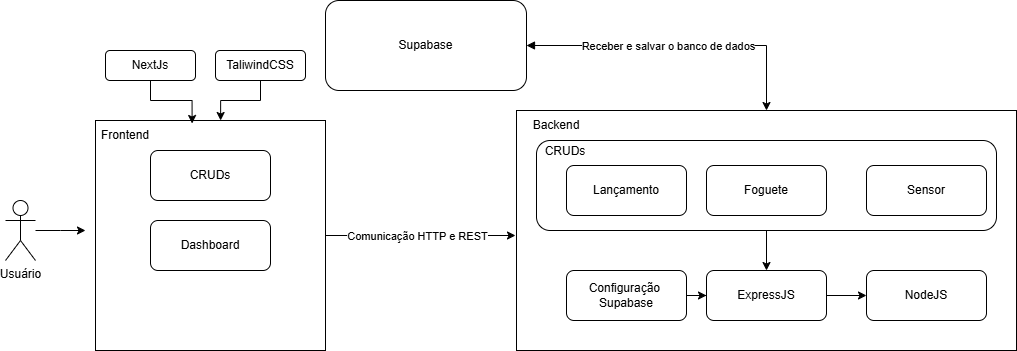
\includegraphics[width=1\linewidth]{editaveis/figuras/diagrama_arquitetura.png}
  \caption{Diagrama Arquitetura}
  \label{fig:enter-label}
\end{figure}



\subsection{Diagrama Entidade Relacionamento}
O DER (Diagrama Entidade-Relacionamento) é uma representação conceitual que mapeia as entidades (objetos do domínio), seus atributos e os relacionamentos, sem detalhes técnicos de implementação. No diagrama fornecido, gerado na ferramenta BrModelo, três entidades principais estruturam o modelo:

\begin{itemize}
  \item \textbf{FOGUETE} (com atributos: \textit{id, nome, peso\_ZFW}) relaciona-se com \textbf{LANÇAMENTO} através do vínculo \textit{"realiza"}, onde:
  \begin{itemize}
    \item Um foguete pode ter múltiplos lançamentos (cardinalidade 1,n);
    \item Cada lançamento pertence a um único foguete (cardinalidade 1,1).
  \end{itemize}

  \item \textbf{LANÇAMENTO} (com atributos: \textit{id, data\_hora, angulo\_inicial, nivel\_agua, pressao\_inicial, massa\_foguete\_total}) relaciona-se com \textbf{DADOCOLETADO} pelo vínculo \textit{"gera"}, onde:
  \begin{itemize}
    \item Cada lançamento produz múltiplos dados (cardinalidade 1,n);
    \item Cada dado está vinculado a um único lançamento (cardinalidade 1,1).
  \end{itemize}

  \item \textbf{DADOCOLETADO} (com atributos: \textit{id, tempo, posicoes, velocidade}) armazena as medições técnicas.
\end{itemize}

\begin{figure}[H]
\centering
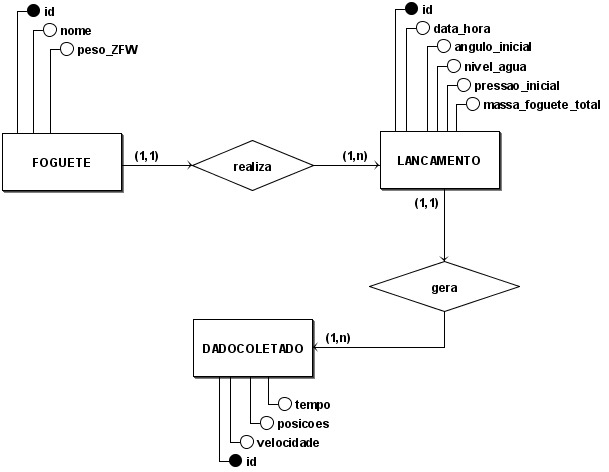
\includegraphics[width=1\linewidth]{editaveis/figuras/diagrama_EntidadeRelacionamento.png}
\caption{Diagrama Entidade Relacionamento}
\label{fig:enter-label}
\end{figure}

\subsection{Diagrama Lógico de Dados}

O DLD (Diagrama Lógico de Dados) é uma etapa fundamental no projeto de bancos de dados, responsável por transformar o modelo conceitual (DER) em uma estrutura técnica preparada para implementação física. Enquanto o DER foca em \textit{"o que"} o sistema precisa armazenar (entidades, atributos e relacionamentos), o DLD define \textit{"como"} esses elementos serão organizados no banco de dados, detalhando: No exemplo gerado com \textbf{BrModelo}, o DLD materializa o DER da seguinte forma:

\begin{itemize}
  \item A tabela \textbf{FOGUETE} contém os atributos: \textit{id} (UUID, chave primária), \textit{nome} (VARCHAR) e \textit{peso\_ZFW} (NUMERIC).
  
  \item A tabela \textbf{LANÇAMENTO} herda os atributos do DER e acrescenta o atributo \textit{foguete\_id} (UUID, chave estrangeira que referencia \textbf{FOGUETE}).

  \item A tabela \textbf{DADOCOLETADO} contém os atributos \textit{id, tempo, posicoes, velocidade} e se vincula à tabela \textbf{LANÇAMENTO} por meio da chave estrangeira \textit{lancamento\_id}.
\end{itemize}

\textbf{Implementação dos Relacionamentos:}
\begin{itemize}
  \item A relação \textit{"um foguete realiza múltiplos lançamentos"} (1,n) é representada pela chave estrangeira \textit{foguete\_id} na tabela \textbf{LANÇAMENTO}.

  \item A relação \textit{"um lançamento gera múltiplos dados"} (1,n) é representada pela chave estrangeira \textit{lancamento\_id} na tabela \textbf{DADOCOLETADO}.
\end{itemize}

\begin{figure}[H]
\centering
\includegraphics[width=1\linewidth]{editaveis/figuras/diagrama_LogicoDados.png}
\caption{Diagrama Lógico de Dados}
\label{fig:dld}
\end{figure}


\renewcommand{\arraystretch}{1.2}

Dicionário de Dados - Projeto Oásis

\subsubsection*{Entidade: FOGUETE}  
\textit{Descrição}: Contém informações dos foguetes utilizados nos lançamentos.  

\begin{longtable}{|p{2.5cm}|p{3.5cm}|p{2cm}|p{1.8cm}|p{4cm}|}
\hline
\textbf{Atributo} & \textbf{Propriedades do Atributo} & \textbf{Tipo de Dado} & \textbf{Tamanho} & \textbf{Descrição} \\
\hline
\endfirsthead

\hline
\textbf{Atributo} & \textbf{Propriedades do Atributo} & \textbf{Tipo de Dado} & \textbf{Tamanho} & \textbf{Descrição} \\
\hline
\endhead

id & Chave primária, obrigatório & UUID & - & Identificador do foguete \\
\hline
nome & Obrigatório & VARCHAR & - & Nome do foguete \\
\hline
peso\_ZFW & Obrigatório & NUMERIC & 10,2 & Peso do foguete sem água (Zero Fuel Weight) \\
\hline
\end{longtable}

\subsubsection*{Entidade: LANCAMENTO}  
\textit{Descrição}: Contém os dados relacionados aos lançamentos de foguetes com água.  

\begin{longtable}{|p{3.7cm}|p{2.7cm}|p{2cm}|p{1.8cm}|p{4cm}|}
\hline
\textbf{Atributo} & \textbf{Propriedades do Atributo} & \textbf{Tipo de Dado} & \textbf{Tamanho} & \textbf{Descrição} \\
\hline
\endfirsthead

\hline
\textbf{Atributo} & \textbf{Propriedades do Atributo} & \textbf{Tipo de Dado} & \textbf{Tamanho} & \textbf{Descrição} \\
\hline
\endhead

id & Chave primária, obrigatório & UUID & 11 & Identificador do lançamento \\
\hline
data\_hora & Obrigatório & DATE & - & Data e hora do lançamento \\
\hline
angulo\_inicial & Obrigatório & REAL & 2 & Ângulo inicial do lançamento \\
\hline
nivel\_agua & Obrigatório & NUMERIC & 300 & Nível de água no momento do lançamento \\
\hline
pressao\_inicial & Obrigatório & REAL & 4 & Pressão inicial no lançamento \\
\hline
massa\_foguete\_total & Obrigatório & NUMERIC & 10,2 & Massa total do foguete \\
\hline
FOGUETE\_id & Chave estrangeira, obrigatório & UUID & - & ID do foguete utilizado no lançamento \\
\hline
\end{longtable}

\subsubsection*{Entidade: DADOCOLETADO}  
\textit{Descrição}: Contém os dados registrados durante o lançamento de um foguete.  

\begin{longtable}{|p{3.7cm}|p{2.7cm}|p{1.6cm}|p{1.8cm}|p{4cm}|}
\hline
\textbf{Atributo} & \textbf{Propriedades do Atributo} & \textbf{Tipo de Dado} & \textbf{Tamanho} & \textbf{Descrição} \\
\hline
\endfirsthead

\hline
\textbf{Atributo} & \textbf{Propriedades do Atributo} & \textbf{Tipo de Dado} & \textbf{Tamanho} & \textbf{Descrição} \\
\hline
\endhead

id & Chave primária, obrigatório & UUID & - & Identificador do dado coletado \\
\hline
LANCAMENTO\_id & Chave estrangeira, obrigatório & UUID & - & ID do lançamento ao qual os dados pertencem \\
\hline
posicoes & Obrigatório & REAL & - & Posição registrada durante o voo \\
\hline
velocidade & Obrigatório & REAL & - & Velocidade registrada durante o voo \\
\hline
tempo & Obrigatório & REAL & - & Tempo registrado correspondente aos dados \\
\hline
\end{longtable}


\subsection{Diagrama de Estados}
O diagrama de estados é um tipo de diagrama utilizado para modelar o comportamento dinâmico de um sistema, descrevendo os diferentes estados que um objeto ou sistema pode assumir ao longo do tempo, bem como os eventos ou condições que causam as transições entre esses estados.

\begin{landscape}
\begin{figure}
    \centering
    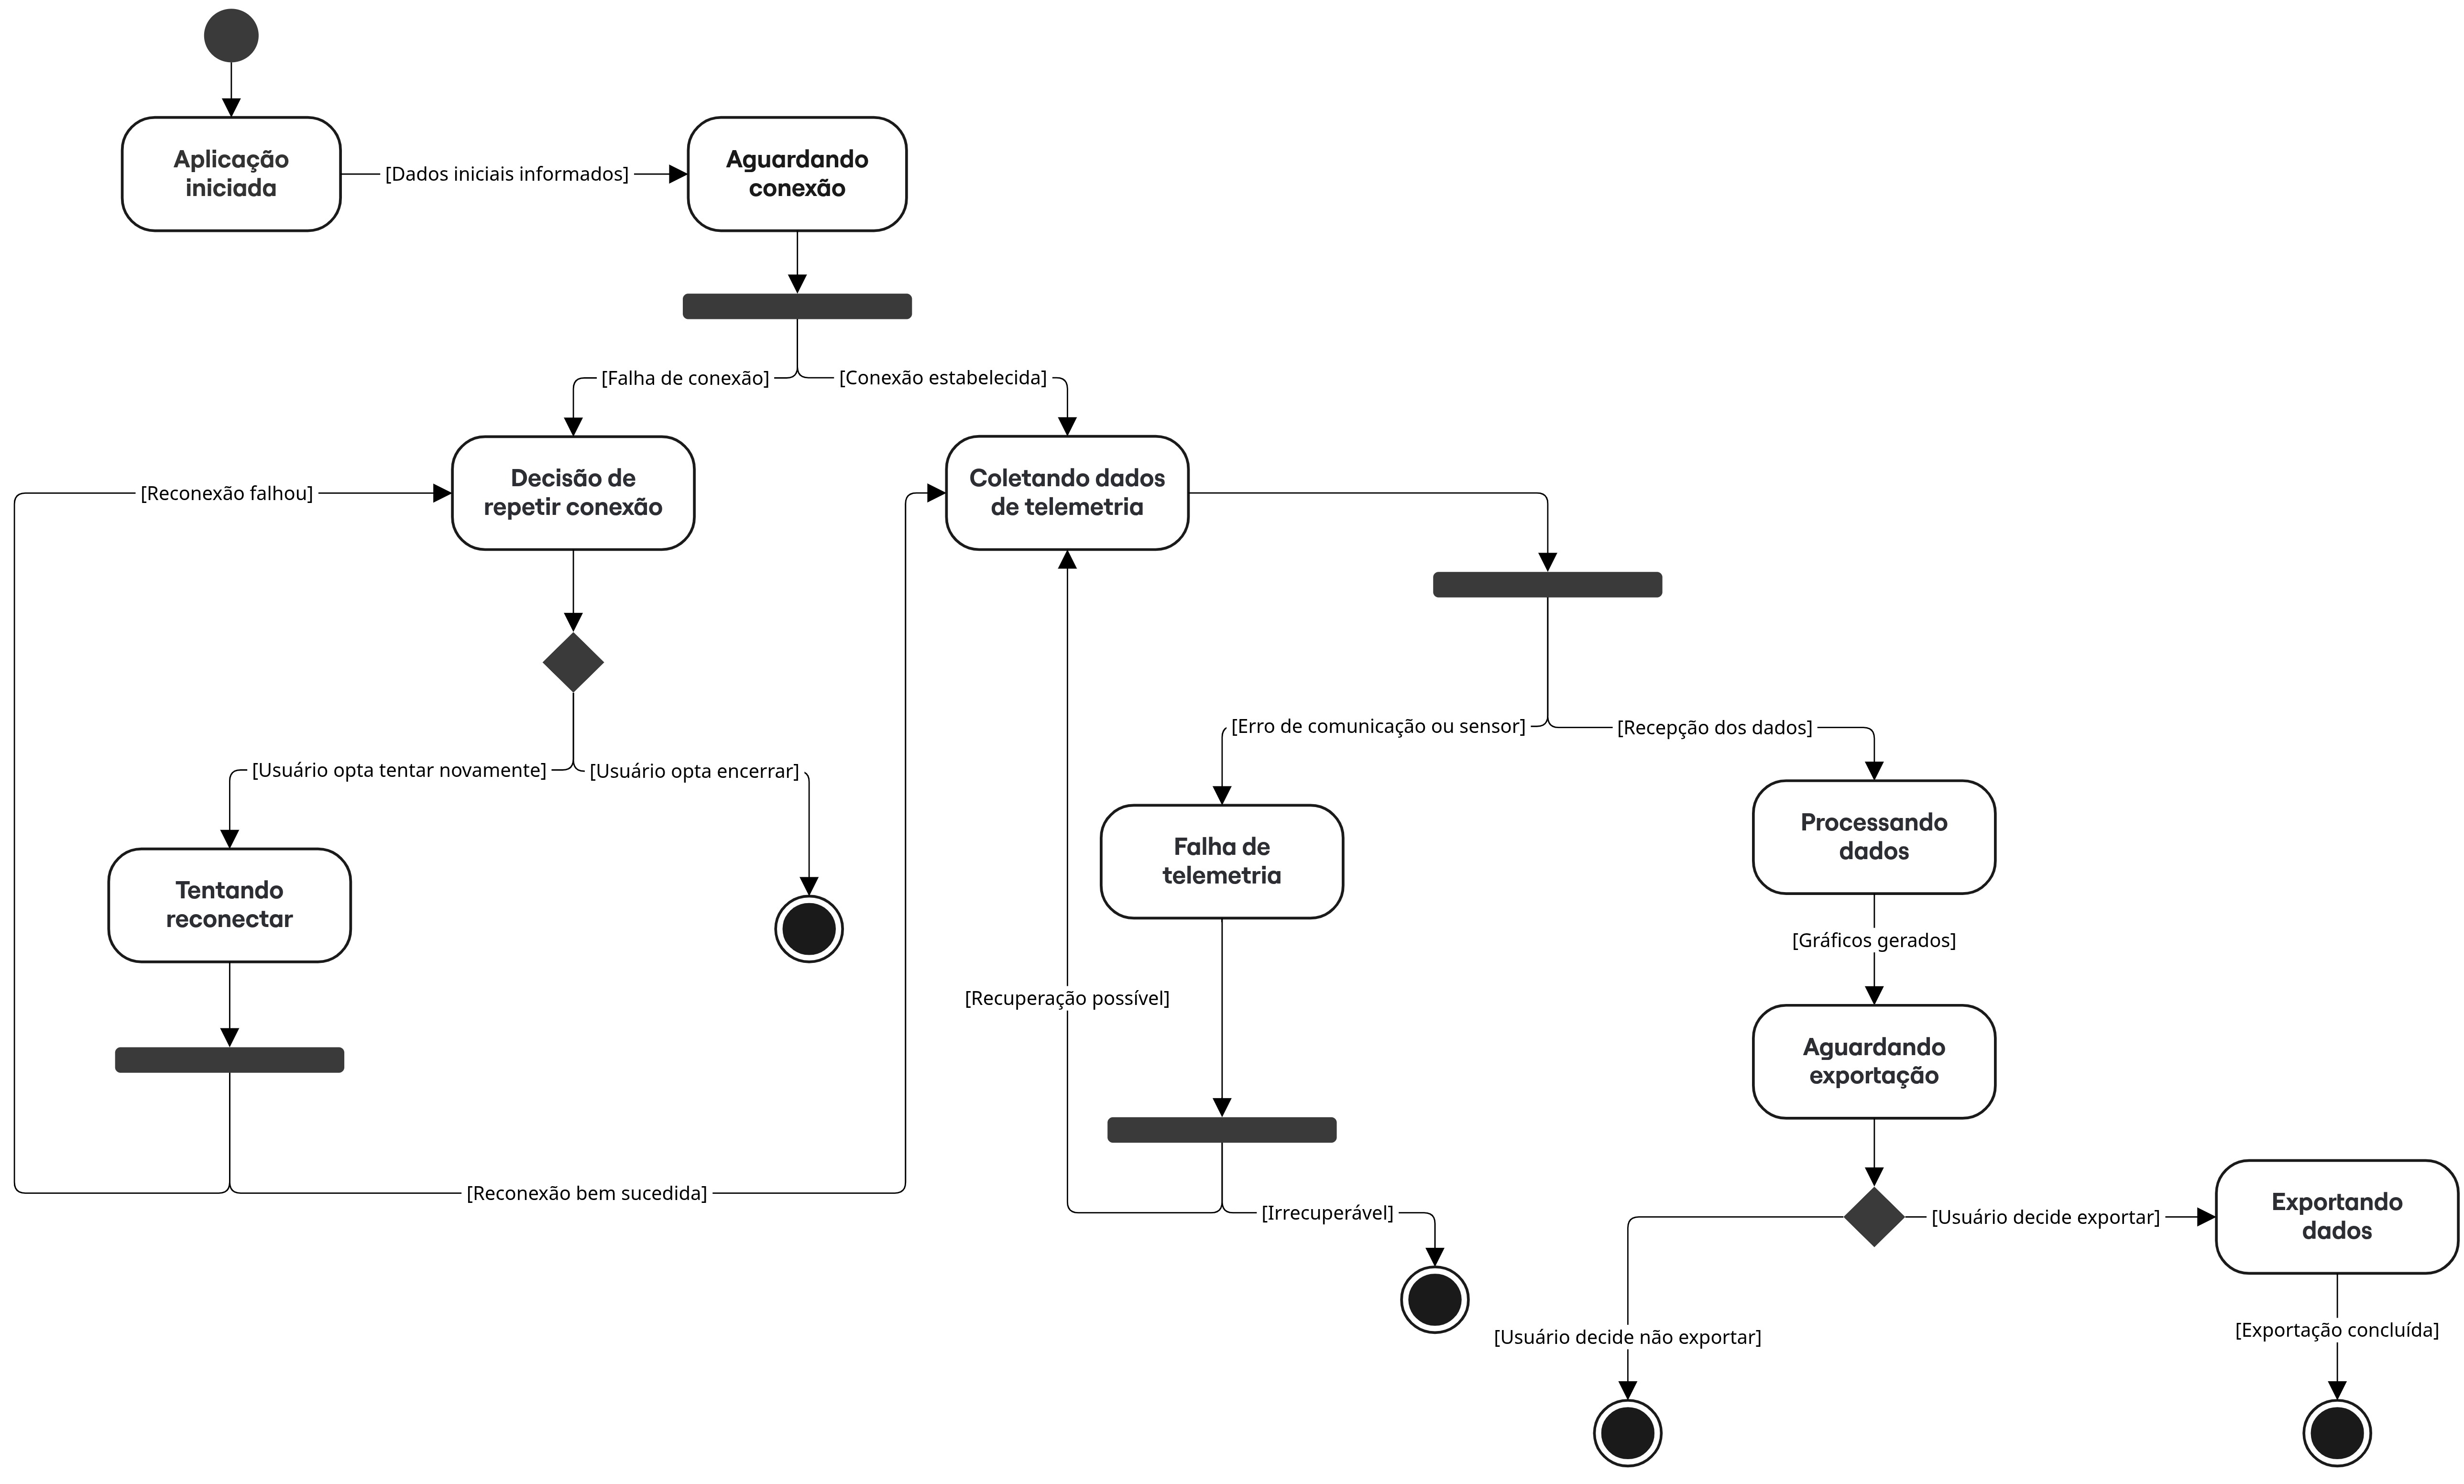
\includegraphics[width=1\linewidth]{editaveis/figuras/diagrama_de_estados.jpg}
    \caption{Diagrama de Estados}
    \label{fig:enter-label}
\end{figure}
\end{landscape}



\textcolor{red}{ \textbf{Protótipo funcional do \textit{software}, navegável.}}

\subsection{Especificações de Caso de Testes}

Os testes de software são fundamentais para assegurar a qualidade e a confiabilidade dos sistemas, atuando como uma barreira crítica contra falhas. Essa prática consiste em executar o programa com o objetivo explícito de identificar erros e verificar se seu comportamento está alinhado aos requisitos especificados. Além de detectar defeitos existentes, os testes ajudam a prevenir problemas futuros, conferindo maior segurança quanto à estabilidade e funcionalidade do produto final.

A especificação de testes formaliza esse processo ao estruturar os cenários de validação em um roteiro claro e sistemático. Ela define as condições de execução, os passos a serem seguidos, as entradas e os resultados esperados para cada caso, servindo como base para avaliar a conformidade com os requisitos do usuário. Para isso, utiliza-se uma tabela de casos de teste, que organiza cada cenário por meio de colunas como ID (identificador único do caso de teste, que permite rastreamento e referência rápida), Objetivo do Teste (descrição clara do que se pretende validar), Pré-condições (estado necessário do sistema antes da execução), Entradas (valores ou ações fornecidos ao sistema), Passos (sequência de ações a serem realizadas), Resultado Esperado (comportamento ou saída que o sistema deve apresentar) e Prioridade (grau de importância do teste, que auxilia na organização da execução). Essa estrutura organizada garante rastreabilidade, cobertura abrangente dos requisitos e validação minuciosa das funcionalidades — elementos essenciais para assegurar a qualidade e a confiabilidade do resultado final.

\subsubsection*{Tabela de Especificação de Casos de Teste - Software}
\begin{longtable}{|p{1cm}|p{2cm}|p{2cm}|p{2.2cm}|p{2cm}|p{2cm}|p{2.1cm}|}
  \hline
  \textbf{ID} & \textbf{Objetivo do Teste} & \textbf{Pré-condições} & \textbf{Entrada} & \textbf{Passos} & \textbf{Resultado Esperado} & \textbf{Prioridade} \\
  \hline
  \endfirsthead
  
  \hline
  \textbf{ID} & \textbf{Objetivo do Teste} & \textbf{Pré-condições} & \textbf{Entrada} & \textbf{Passos} & \textbf{Resultado Esperado} & \textbf{Prioridade} \\
  \hline
  \endhead
  
  CT01 & Verificar inicialização da aplicação & Sistema instalado & Nenhuma & Iniciar o sistema & Tela inicial da aplicação é exibida & Alta \\
  \hline
  CT02 & Validar entrada de dados iniciais & Aplicação iniciada & Pressão, volume e ângulo & Inserir dados e confirmar entrada & Dados são aceitos e armazenados & Alta \\
  \hline
  CT03 & Verificar conexão com servidor embarcado & Dados iniciais inseridos & Nenhuma & Clicar em conectar e aguardar resposta & Sistema conecta ao servidor e exibe confirmação & Alta \\
  \hline
  CT04 & Testar reconexão após falha & Conexão inicial falhou & Opção de tentar novamente & Selecionar “tentar novamente” e aguardar reconexão & Reconexão realizada com sucesso ou tentativa encerrada & Média \\
  \hline
  CT05 & Validar coleta de dados & Conectado ao servidor & Nenhuma & Iniciar coleta e aguardar leitura de dados & Dados são recebidos com sucesso & Alta \\
  \hline
  CT06 & Testar falha na coleta & Conectado ao servidor & Comunicação interrompida ou erro & Iniciar coleta e simular erro & Sistema detecta falha e informa ao usuário & Alta \\
  \hline
  CT07 & Verificar salvamento de dados no banco & Dados coletados com sucesso & Nenhuma & Finalizar coleta e aguardar confirmação & Dados persistidos corretamente no banco & Alta \\
  \hline
  CT08 & Gerar gráficos com dados salvos & Dados salvos no banco & Nenhuma & Solicitar geração de gráficos & Gráficos são exibidos na tela & Alta \\
  \hline
  CT09 & Visualizar gráficos & Gráficos gerados & Nenhuma & Acessar seção de visualização & Gráficos são exibidos de forma clara & Alta \\
  \hline
  CT10 & Exportar dados & Dados disponíveis & Seleção de tipo de exportação & Escolher “exportar dados”, selecionar formato e confirmar & Processo de exportação iniciado & Média \\
  \hline
  CT11 & Exportar dados como PDF & Dados disponíveis & Selecionar exportação PDF & Iniciar exportação, selecionar “PDF” e confirmar & Arquivo PDF é gerado corretamente & Baixa \\
  \hline
  CT12 & Exportar dados como CSV & Dados disponíveis & Selecionar exportação CSV & Iniciar exportação, selecionar “CSV” e confirmar & Arquivo CSV é gerado corretamente & Baixa \\
  \hline
  \end{longtable}

% \section{Estrutura}

% \textcolor{red}{Apresentar desenho em CAD, indicar dimensões por lado/aresta/cota, indicar materiais utilizados e explicar o desenho e as decisões de projeto.}

% \section{Descrição de \textit{hardware}}

% \textcolor{black}{A descrição de hardware deste documento foi elaborada para garantir a replicabilidade do sistema, seguindo padrões técnicos e organizacionais claros. Para isso, são apresentados três elementos fundamentais: }

% \textcolor{black}{\begin{itemize}
%     \item O diagrama de blocos \cite{blockdiagram}: Oferece uma visão geral da arquitetura, destacando a interação entre sensores, atuadores, núcleo de controle e subsistemas de alimentação, com as principais partes do sistema e as ligações entre elas.
%     \item A lista de materiais \cite{bom}: que facilita a montagem do sistema a partir da escolha dos componentes, quantidades e custos, permitindo o planejamento financeiro e a aquisição precisa de itens.
%     \item O esquemático \cite{esquematico}: Detalha as conexões físicas entre os elementos, incluindo pinagem, protocolos de comunicação e proteção de circuitos.
% \end{itemize}}

% \textcolor{black}{Além disso, as justificativas técnicas embasam as escolhas dos componentes, garantindo que cada decisão esteja alinhada com os requisitos de desempenho, segurança e custo-benefício. Essa estrutura permite não apenas a reprodução fiel do projeto, mas também sua adaptação para cenários alternativos, como a inclusão de novos sensores ou a otimização de consumo energético. }

% \section{Análise de consumo energético}

% Nessa seção, faremos a modelagem matemática do projeto, analisando objetivos, estrutura, movimento e trajetória. Nesse primeiro momento, ao analisar o movimento cinemático do foguete, utilizaremos a referência \cite{moyses}.

%  Tendo em vista o objetivo de atingir um alcance máximo de 30 metros, definimos então que num ângulo de lançamento de 45° o foguete deve atingir os 30 metros de alcance, uma vez que esse é o ângulo de alcance máximo para o lançamento de um projétil.  Analisando as componentes vertical e horizontal do movimento do foguete, vamos encontrar o tempo necessário para que ele realize o movimento completo:
% \begin{equation}
%     v=v_{oy}+\frac{at}{2} \xrightarrow{} 0=v_{oy}-\frac{9,81t}{2}\xrightarrow{}v_{oy}=\frac{9,81t}{2},
%     \label{componente vertical}
% \end{equation}
% \begin{equation}
%     s=s_o+v_{ox}.t \xrightarrow{} 30=v_{ox}.t \xrightarrow{} v_{ox}=\frac{30}{t}.
%     \label{componente horizontal}
% \end{equation}

% Note que na equação \ref{componente vertical}, o tempo t é dividido por 2, uma vez que essa componente da velocidade zera o seu valor ao chegar na altura máxima, ou seja, na metade da trajetória.

% Considerando que o ângulo de lançamento para esse caso é de 45°, as componentes \(v_{ox}\) e \(v_{oy}\) são numericamente iguais, portanto:
% \begin{equation}
%     \frac{30}{t}=\frac{9,81t}{2} \xrightarrow{} t^2=\frac{30.2}{9,81} \xrightarrow{} t \approx 2,5s.
%     \label{tempo t}
% \end{equation}

% A partir disso, encontramos, também, a velocidade inicial necessária do foguete:

% \begin{equation}
%      v_o.cos 45°=v_{ox} \xrightarrow{} v_o= \frac{v_{ox}.2}{\sqrt{2}}\xrightarrow{} v_o=\frac{\frac{30}{t}2}{\sqrt{2}} \xrightarrow{} v_o \approx 17 m/s.
%      \label{vo}
% \end{equation}

% Agora que analisamos o movimento cinemático do projeto, partimos para a dinâmica, ou seja, tudo aquilo que causa o movimento do foguete. Para esse cálculo analítico, utilizaremos a referência \cite{rocketpropulsionelements}.
% Encontramos primeiramente, a velocidade de escape da água, por meio da equação do foguete. Entretanto, são necessários os parâmetros de massa do foguete, ou seja, a massa inicial do foguete com água e a massa final dele, depois de todo o impulso dado. Para esses parâmetros faremos uma estimativa a partir dos cálculos e dados experimentais encontrados em \cite{tcc}, onde, para o nosso objetivo, a razão de massas é de aproximadamente 6. Encontramos, então, a velocidade de escape da água:
% \begin{equation}
%     \Delta V=v_o= v_e.\ln{\frac{m_o}{m_f}}.
%     \label{ve}
% \end{equation}
% \begin{equation}
%     v_e=\frac{\Delta V}{\ln{\frac{m_o}{m_f}}} \xrightarrow{} v_e=\frac{17}{ln{6}} \approx 9,5 m/s.
% \end{equation}
% Sabendo a velocidade de escape, podemos, por meio da equação de Bernoulli, considerando o fluxo ideal e incompressível e a densidade da água de 1000 \(kg/m^3\) , encontrar a pressão manométrica do foguete, ou seja, a pressão necessária dentro da cápsula de ar para o alcance da missão.

% \begin{equation}
%     P_o+\frac{\rho. v^2}{2}=P+\frac{\rho . v_e^2}{2} \xrightarrow{} \Delta P=\frac{\rho.v_e^2}{2} - \cancel{\frac{\rho.v^2}{2}} \xrightarrow{} \Delta P=\frac{1000.9,5^2}{2} \approx 45125 Pa.
%     \label{delta P}
% \end{equation}

% Calculamos, então, o fluxo de massa de água, por meio de:
% \begin{equation}
%     \dot{m}=\rho.A.v_e
%     \label{mponto}
% \end{equation}
% em que A é a área de saída da água. Estimando a área de saída da garrafa como aproximadamente 5 \(cm^2\), encontramos o seguinte resultado de fluxo de massa:
% \begin{equation}
%     \dot{m}=1000.5.10^{-4}.9,5 \approx 4,75kg/s.
% \end{equation}
% Calculamos então o empuxo necessário:
% \begin{equation}
%     T=\dot{m}.v_e=4,75.9,5=45N
%     \label{empuxo}
% \end{equation}

% Por fim, baseado na teoria proposta pela referência \cite{rocketpropulsionelements}, e considerando que o "tempo de queima", ou seja, o tempo de duração que a água vai ser expelida seja 1/10 do tempo da trajetória, encontramos o impulso total necessário:
% \begin{equation}
%     I_t=T.\Delta t =45.0,25=11,25N.s
%     \label{impulso total}
% \end{equation}

% E, finalmente, calculamos o consumo de água do foguete para um alcance de 30 metros:
% \begin{equation}
%     Q_{agua}=4,75.0,25=1,1875L .
%     \label{quantidade de agua}
% \end{equation}

% Para os outros alcances, vamos variar apenas a pressão necessária no compartimento, ou seja, manteremos o ângulo de lançamento. Repetimos o processo dos cálculos para um alcance de 10 m e 20 m.


% \begin{table}[h!]
% \centering
% \begin{tabular}{llllllllll}
% Alcance & t & $t_q$ & $v_o$ & $v_e$ & $\dot{m}$ & T & $I_t$ & $\Delta P$ & $Q_{agua}$ \\
% 10m & 1,45s & 0,145s & $9,75m/s$ & $5,45m/s$ & $2,72kg/s$ & 14,8N & 2,15N.s & 14851Pa & 0,4L \\
% 20m & 2,04s & 0,204s & $13,86m/s$ & $7,75m/s$ & $3,88kg/s$ & 30N & 6,12N.s & 30031Pa & 0,8L
% \end{tabular}
% \end{table}


% Foi feito o mesmo passo a passo das contas feitas para um alcance de 30 metros, considerando \(t_q\) o suposto "tempo de queima", utilizando as seguintes equações: equação \ref{tempo t} para o tempo t, equação \ref{vo} para o \(v_o\), equação \ref{ve} para o cálculo do \(v_e\), equação \ref{mponto} para o cálculo do \(\dot{m}\), equação \ref{empuxo} para o cálculo de T, equação \ref{impulso total} para o cálculo do \(I_t\), equação \ref{delta P} para o cálculo do \(\Delta P\) e, por fim, equação \ref{quantidade de agua} para o cálculo do \(Q_{agua}\).

% Para garantir o funcionamento eficiente do sistema eletrônico no foguete de água, é fundamental realizar uma análise do consumo energético. 	Como o projeto envolve diversos componentes eletrônicos com exigências distintas de tensão e corrente, será utilizado um regulador de tensão. Esse dispositivo permitirá adaptar a tensão fornecida pela bateria às necessidades específicas de cada parte do circuito, assegurando a integridade e o desempenho ideal. 

% Para  analisar a potência consumida em cada componente individualmente, será considerado o consumo médio da corrente e a tensão ideal. A forma utilizada para o cálculo é:
% \begin{equation}
%     P = V \cdot I 
% \end{equation}

% onde P é a potência (em watts), V é a tensão (em volts), e I a corrente elétrica (em amperes)

% A partir dos dados obtidos, será possível estimar o consumo total do sistema e, com isso, selecionar uma bateria que ofereça a tensão adequada e capacidade suficiente para garantir a autonomia e o funcionamento seguro durante toda a operação do foguete.

% \begin{figure}[H]
%     \centering
%     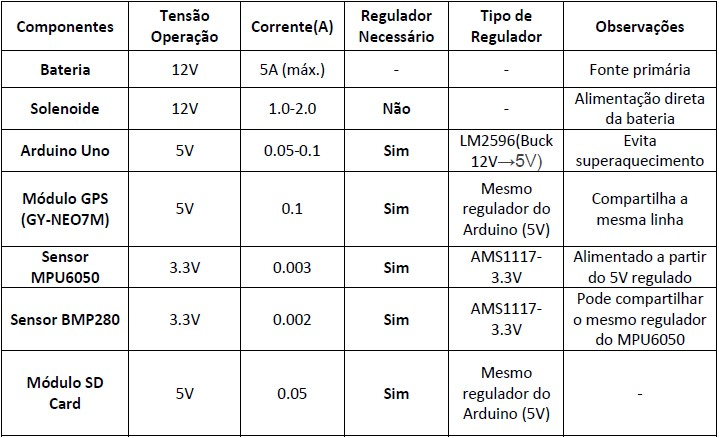
\includegraphics[width=0.75\textwidth]{figuras/Tabela.jpg}
%     \label{fig:tabela}
% \end{figure}

% \noindent Esquema de Conexões:

% \begin{figure}[H]
%     \centering
%     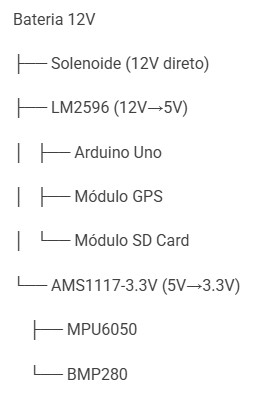
\includegraphics[width=0.3\textwidth]{figuras/Esquema.jpg}
%     \label{fig:tabela}
% \end{figure}


% \noindent Cálculo de autonomia:
% \begin{itemize}
%     \item Energia da Bateria
%     \item $12V \cdot5Ah = 60 Wh (216.000J)$
%     \item Consumo por lançamento: ~242J (incluindo solenoide)
%     \item Lançamentos possíveis:
% \end{itemize}
% \quad \qquad 216.000J/242J/lançamento = 216.000J $\approx$ 892 lançamentos



% \section{Descrição de \textit{software}}

% \textcolor{red}{Com relação ao \textit{software}, será necessário apresentar os seguintes itens: % pacotes de componentes de \textit{software}, suas funções e características, e explicar as decisões de projeto:
% \begin{enumerate}
%     \item Um diagrama do processo de negócio do problema que a máquina se propõe a resolver (BPNM) – não é UML, mas é fundamental para entender como o sistema se comporta como um todo, incluindo o usuário;
%     \item Lista de casos de uso (backlog do sistema). Backlog funcional;
%     \item Lista de requisitos não-funcionais a serem satisfeitos pelo sistema;
%     \item Diagrama de casos de uso: mostrando os requisitos funcionais, seus atores e como eles interagem entre si;
%     \item Diagrama de Classes: apresentando quais dados são manipulados pelo sistema (internamente e externamente – ex.: resultados de experimentos);
%     \item Diagrama de arquitetura, identificando todos os componentes da máquina e suas iterações com o software;
%     \item Diagrama de estados da máquina (sistema);
%     \item Descrição dos testes dos componentes da máquina e dos testes funcionais que deveriam ser feitos para avaliar o funcionamento da máquina e identificar defeitos. São importantes os testes unitários (componentes) e de integração (conjunto de componentes) e o roteiro de testes.
% \end{enumerate}
% }
% %\textcolor{red}{Com relação ao \textit{software}, será necessário apresentar pacotes de componentes de \textit{software}, suas funções e características, e explicar as decisões de projeto.}

